\documentclass[e4_tp2_main.tex]{subfiles}
\begin{document}
\newgeometry{top=2.5cm, bottom=2.0cm, left=2.25cm, right=2.25cm}

\section{Modulación PWM y realimentación}

\begin{figure}[H]
\centering
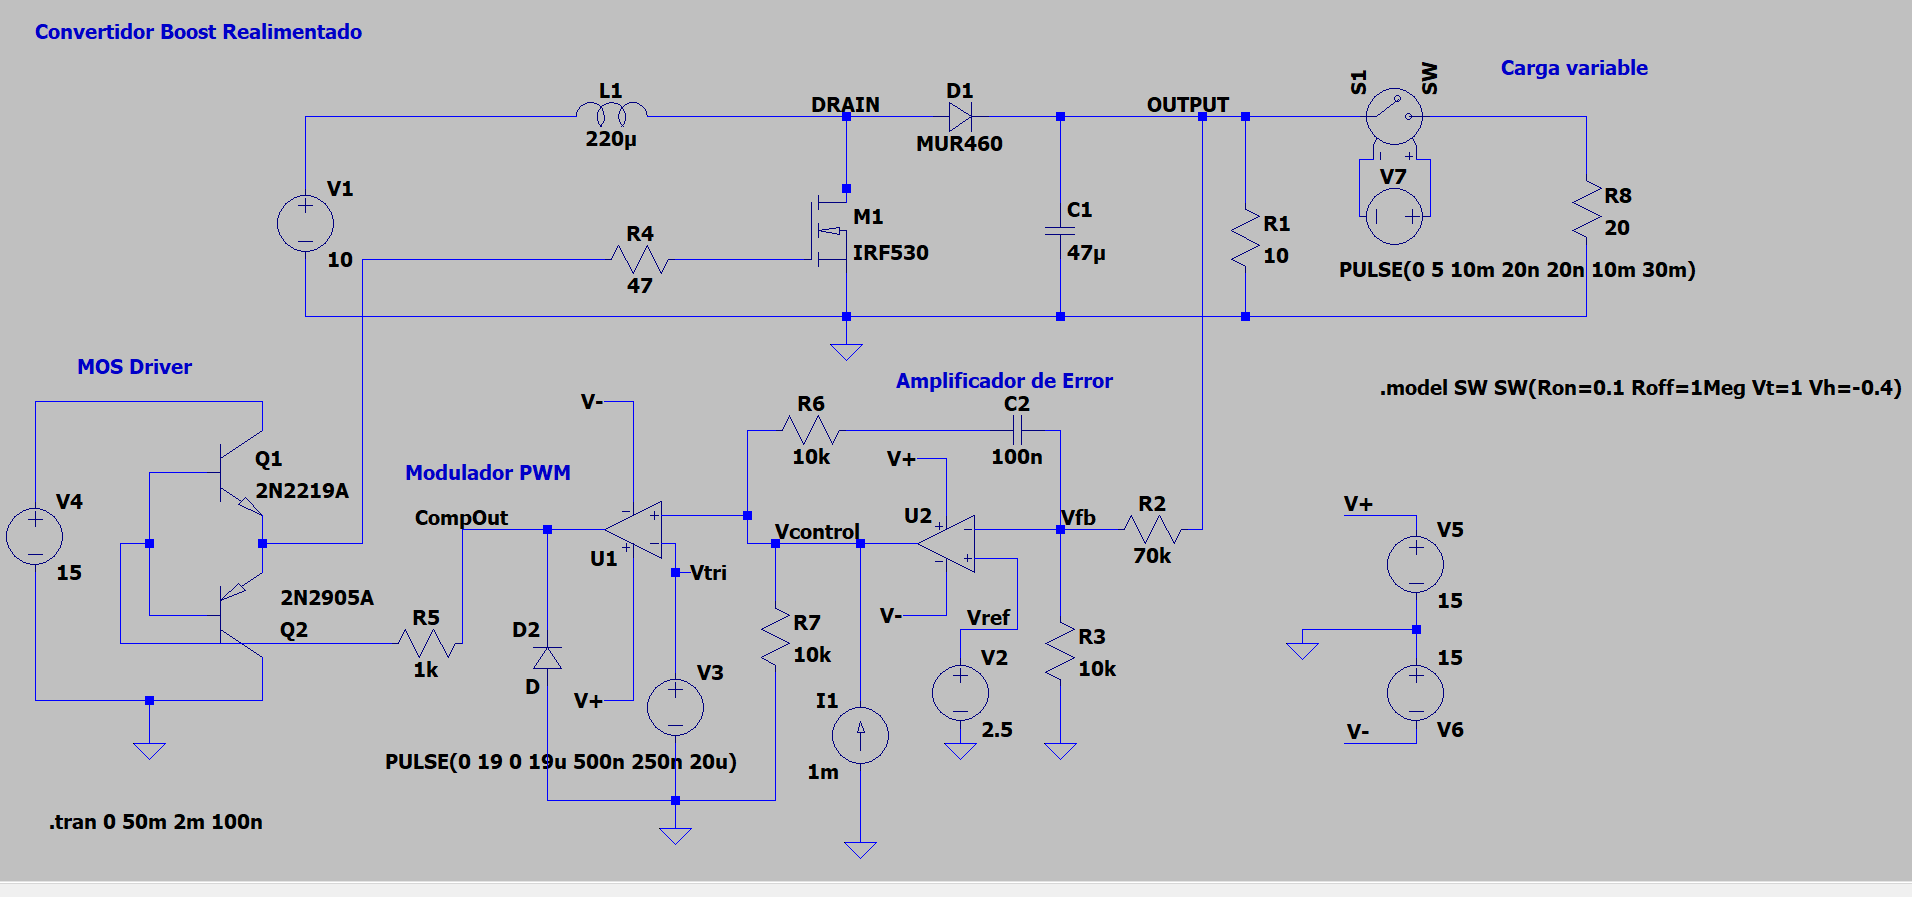
\includegraphics[width=0.9\linewidth]{Imagenes/Punto1/circuito1.png}
\caption{Circuito realimentado a analizar}
\end{figure}

\subsection{Amplificador de error}

\subsubsection*{a) Valores de $R2$ y $R3$ si $V_o=25 VDC$}

Como $V_{FB}$ es el divisor de tensi\'on de $V_o$ y se busca cumplir $V_{FB}=V_{REF}$, se obtiene:

\begin{equation}
V_{FB}=V_{REF}= V_o \cdot \frac{R_3}{R_2+R_3} 
\label{ec1.1.a1}
\end{equation}


Depejando de la ecuaci\'on \eqref{ec1.1.a1} y suponiendo que $R_3=10k \Omega $, obtenemos:

\begin{equation}
R_2=R_3 \cdot \left( \frac{V_o}{V_{REF}} - 1 \right)=90k \Omega \label{ec1.1.a2}
\end{equation}

\subsubsection*{b) Transferencia  $\frac{ \widetilde{v_c}(s)}{\widetilde{v_o}(s)}$ para pequeñas variaciones} 

La transferencia a pequeñas variaciones del amplificador de error se obtiene analizando el inversor con $Z_1=R_2$ y $Z_2=R_6 + \frac{1}{s \cdot C_2}$. Esto se debe a que a pequeñas variaciones, tanto la fuente de tensi\'on $V_2$ como la fuente de corriente $I_1$ se pasivan.

\begin{equation}
\frac{\widetilde{v_c}(s)}{\widetilde{v_o}(s)}=-\frac{R_6 + \frac{1}{s \cdot C_2} }{R_2}  \label{ec1.1.b}
\end{equation}

\subsubsection*{c) Amplificador de error como bloque de un sistema LTI. Ganancia, Polos y Ceros}

Reacomodando la ecuaci\'on \eqref{ec1.1.b}, el diagrama en bloque resulta: 

\begin{center}
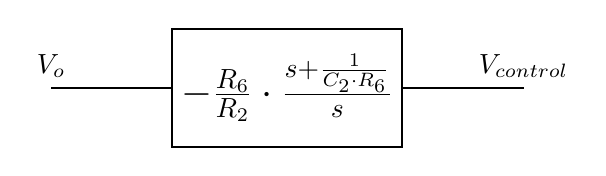
\begin{tikzpicture}[
squarednode/.style={rectangle, draw=black, fill=white!5,thick, minimum size=15mm},
]
\draw[thick] (-3,0) node[above] {$V_{o}$} -- (3,0) node[above] {$V_{control}$};
\node[squarednode]      (maintopic) {\Large {$- \frac{R_6}{R_2} \cdot \frac{s+\frac{1}{C_2 \cdot R_6}}{s}$}};
\end{tikzpicture}
\end{center}


El amplificador de error cuenta con una ganacia $G_{amp}=\frac{R_6}{R_2} =\frac{1}{9}$, un polo en $f_p=\frac{1}{2 \pi \cdot C_2 \cdot R_6 }=159.15Hz$ y un cero en el origen.


\subsubsection*{d) Conjunto fuente de corriente I1 y R7}
La fuente de corriente $I_1$ genera sobre la resistencia $R_7$ una ca\'ida de tensi\'on que marca el punto de operaci\'on con que queremos trabajar. En el caso del circuito que estamos analizando, esa tensi\'on es $V_{control}=10k\Omega \cdot 1mA =10V$. 

Cuando se compara $V_{FB}$ con $V_{REF}$ a la entrada del amplificador de error, se obtiene una diferencia. Dicha diferencia es la que nos determina cu\'anto nos movemos del punto de operaci\'on antes mencionado. Se trabaja alrededor de ese punto porque es el que nos determina el duty requerido a la salida.

\subsection{Modulaci\'on PWM}


\subsubsection*{a) Caracter\'isticas de la se\~nal triangular}
Como podemos observar, la señal que se le inserta en el terminal negativo al amplificador U1 es una señal triangular con un período de 20$\mu $s (50kHz) y una tensión pico $V_p=19 V$. Posee un tiempo de rise $t_r=19 \mu s$ y un tiempo de caída $t_f=500ns$. Con estos valores, podemos establecer que tiene un duty cicle de: $d_{Triang}= \frac{t_r}{T}=0.95$. 
\begin{figure}[H]
\centering
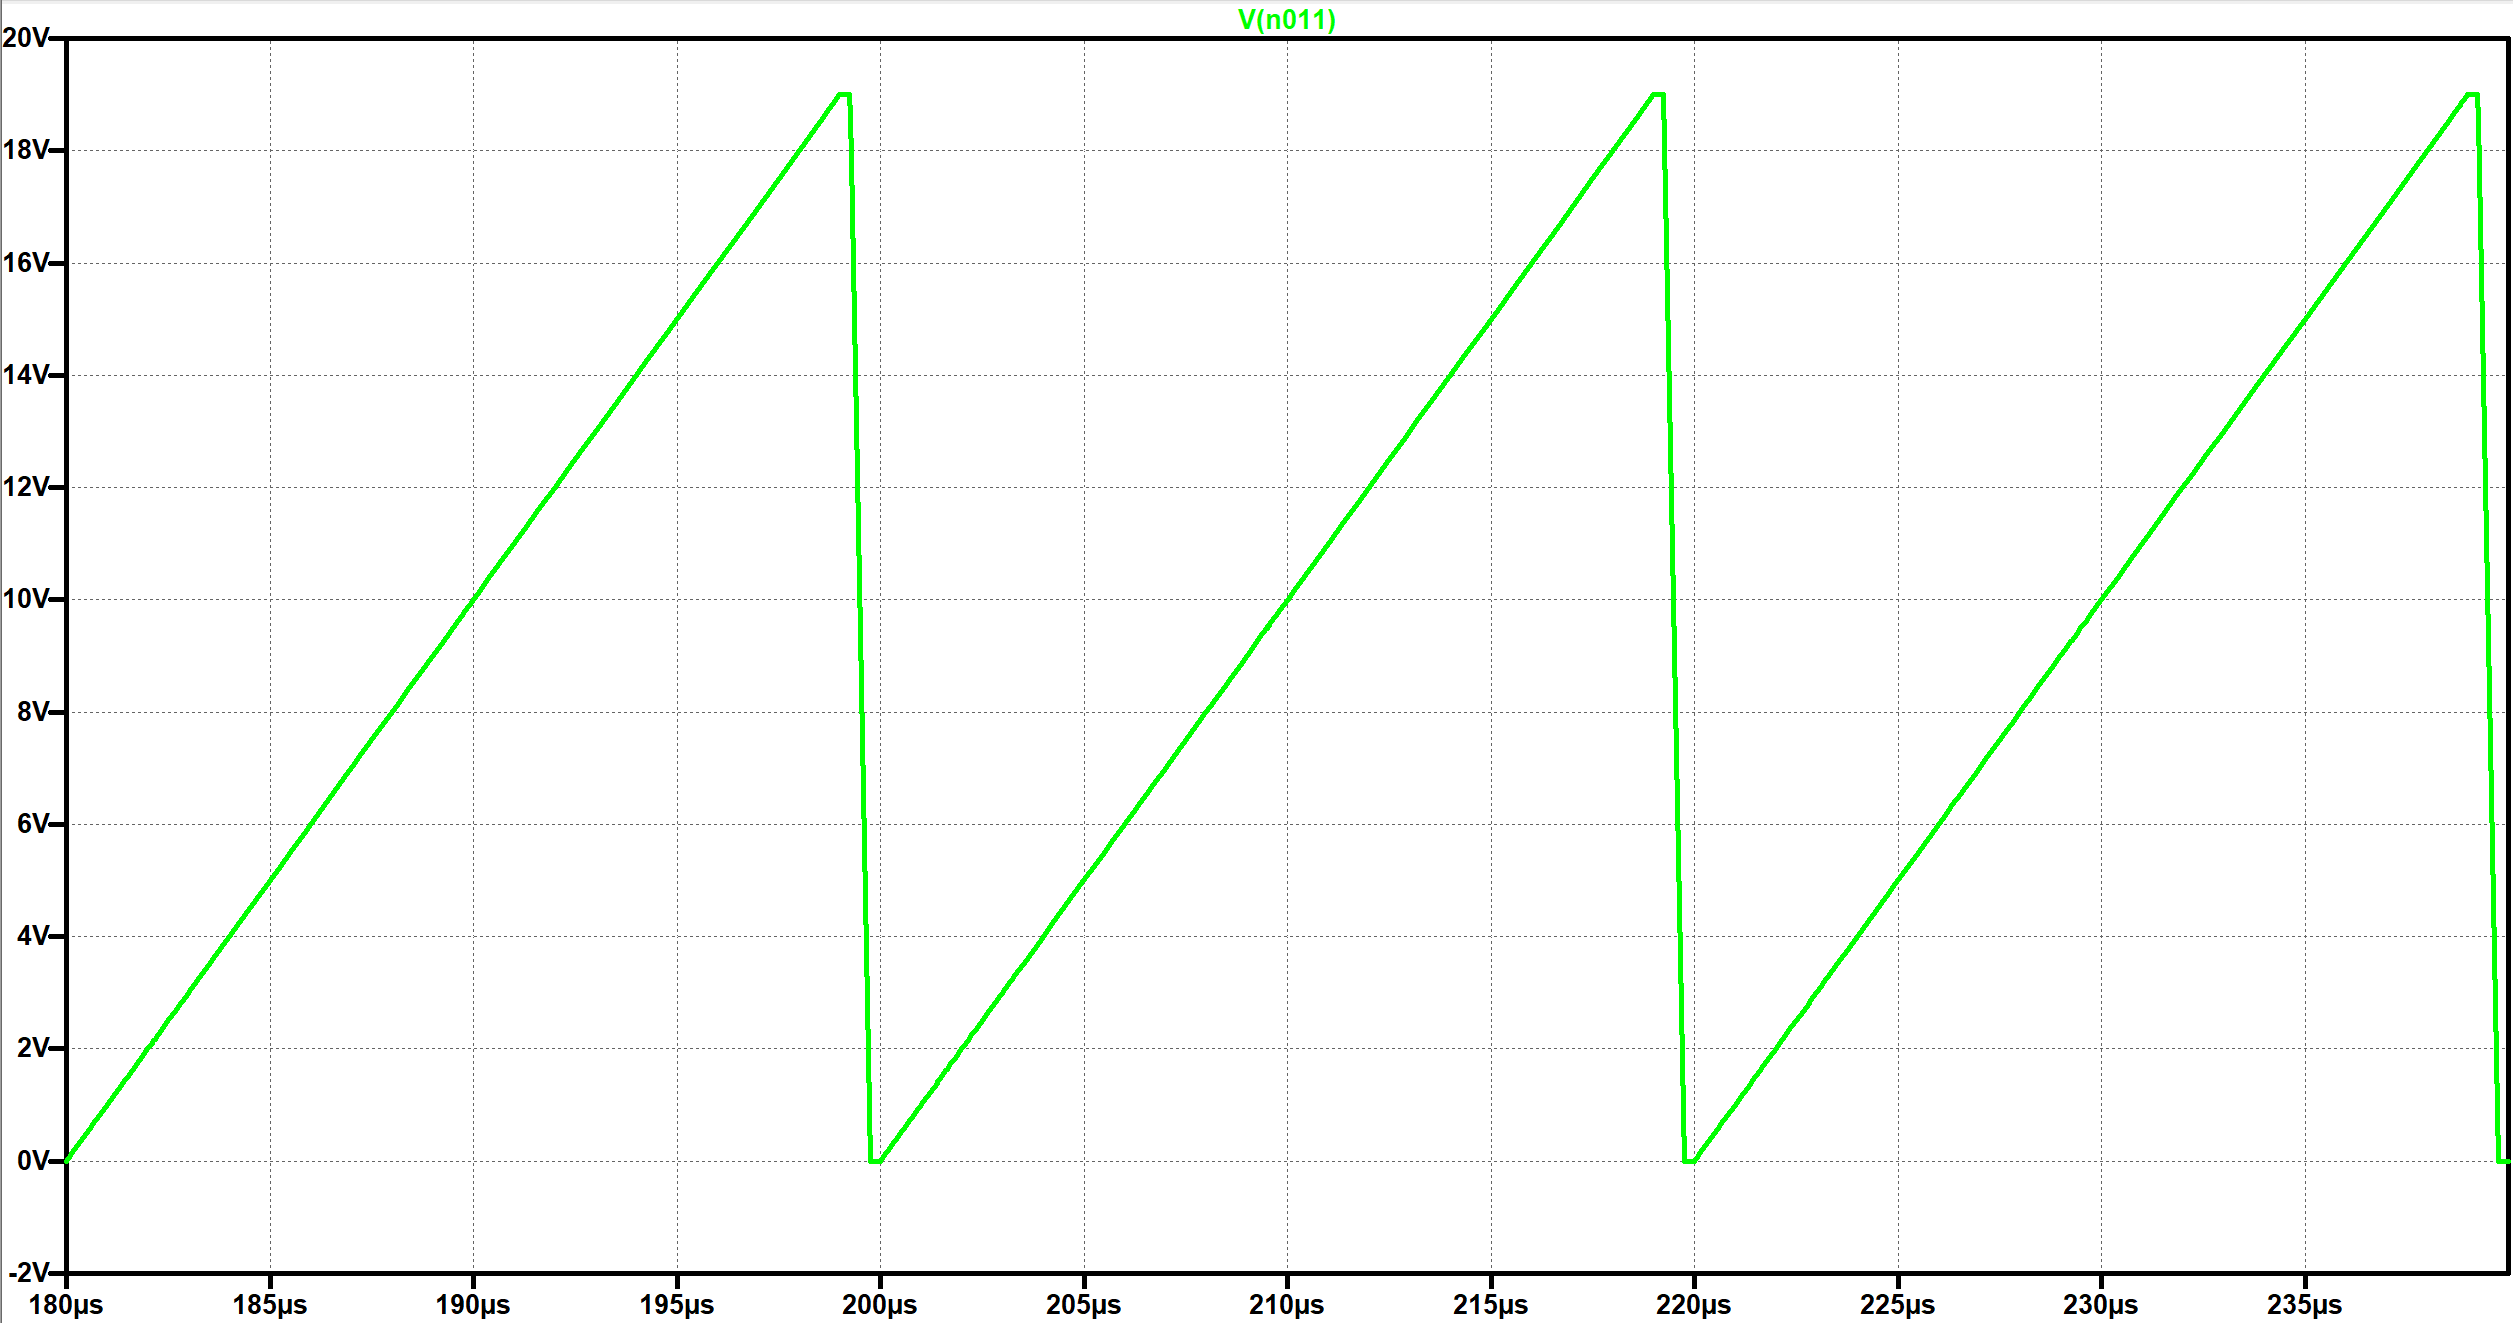
\includegraphics[width=0.4\linewidth]{Imagenes/Punto1/triang_shape.png}
\caption{Señal triangular.}
\end{figure}

\subsubsection*{b) Duty cycle m\'aximo}
Para obtener el duty cycle máximo que puede obtener CompOut, debemos primero calcular la tensión de la señal triangular en el tiempo. Dicha tensión se puede expresar de la siguiente manera:
\begin{equation}
V_{Triang}(t)= \frac{V_{max_{Triang}}}{T_s} \cdot t
\end{equation} 
Sabiendo que el duty cycle es $ d=\frac{t}{T_s}$  , y que el máximo duty se da cuando la tensión de la señal triangular es igual a la tensión de saturación del amplificador, la ecuación queda de la siguiente manera:
\begin{equation}
V_{sat_{Opamp}}= d_{max} \cdot V_{maxtriang} \hspace{0.5cm} \Rightarrow  \hspace{0.5cm} d_{max}= \frac{V_{sat_{Opamp}}}{V_{max_{Triang}}}=\frac{15 V}{19V}=0.79
\end{equation}
\subsubsection*{c) Modulador PWM como bloque de un sistema LTI.}
Para modelar el PWM como un bloque de un sistema LTI, primero debemos hallar su transferencia $\frac{d}{V_{control}}$. Partiendo de la ecuación previa de la diente de sierra, podemos despejar el tiempo y, dividiendo por el período de la señal, encontramos la siguiente transferencia:
\begin{equation}
\frac{d}{V_{control}}=\frac{1}{V_{max_{Triang}}}=\frac{1}{19}
\end{equation} 

De esta forma, el bloque queda conformado de la siguiente forma:

\begin{center}
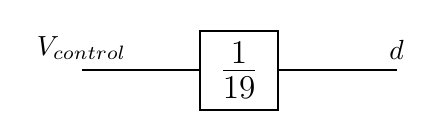
\begin{tikzpicture}[
squarednode/.style={rectangle, draw=black, fill=white!5,thick, minimum size=10mm},
]
\draw[thick] (-2,0)  node[above] {$V_{control}$} -- (2,0) node[above] {$d$};

\node[squarednode]      (maintopic) {\LARGE {$ \frac{1}{19}$}};
\end{tikzpicture}
\end{center}



\subsection{Convertidor DC/DC}
\subsubsection*{a) Funci\'on transferencia del convertidor}

Considerando el diodo y el MOS como ideales, comenzamos analizando el espacio de estados. 

Durante el tiempo que la llave se encuentra cerrada (SW=ON) obtenemos:

\begin{equation}
\underbrace{
\begin{bmatrix}
\dot{i_{L_1}} \vspace{0.2cm} \\
\dot{V_{C_1}} 
\end{bmatrix}
}_{\dot{X}}
=
\underbrace{
\begin{bmatrix}
{0} & {0} \vspace{0.2cm}\\
{0} & {-\frac{1}{R_L \cdot C_1}} 
\end{bmatrix}
}_{A_{on}}
\underbrace{
\begin{bmatrix}
{i_{L_1}} \vspace{0.2cm}\\
{V_{C_1}} 
\end{bmatrix}
}_{X}
+
\underbrace{
\begin{bmatrix}
{\frac{1}{L_1}} \vspace{0.2cm}\\
{0} 
\end{bmatrix}
}_{B_{on}}
V_1
\end{equation}


\begin{equation}
V_o =
\underbrace{
\begin{bmatrix}
{0} & {1} 
\end{bmatrix}
}_{C_{on}}
\begin{bmatrix}
{i_{L_1}} \\
{V_{C_1}} 
\end{bmatrix}
\end{equation}

Por otro lado, durante el tiempo que la llave se encuentra abierta (SW=OFF), se obtiene que: 

\begin{equation}
A_{off} = 
\begin{bmatrix}
{0} & {- \frac{1}{L_1}} \vspace{0.3cm}\\ 
{\frac{1}{C}} & {-\frac{1}{R_L \cdot C_1}}
\end{bmatrix}  
\hspace{2cm} B_{off}=B_{on}  
\hspace{2cm} C_{off} = C_{on}
\end{equation}


A continucaci\'on se calcula el promedio ponderado de las matrices de estado:

\begin{equation}
\overline{A} = A_{on} \cdot d + A_{off} \cdot (1-d) \hspace{2cm} \overline{B}=B_{on} = B_{off}  \hspace{2cm} \overline{C}=C_{on} = C_{off}  
\end{equation}

Finalmente, utilizando la ecuaci\'on provista por la c\'atedra en la clase de Transferencias y reemplazando los valores obtenidos anteriormente obtenemos la transferencia deseada. 

\begin{equation}
\frac{ \widetilde{v_o}(s)}{\widetilde{d}(s)}= \overline{C} \cdot (s \cdot I - \overline{A})^{-1} \left[ (A_{on} - A_{off})X(s) + (B_{on} - B_{off}) V_1 \right] +(C_{on} - C_{off})X(s) 
\label{ec1.3}
\end{equation}

Donde X(s) es el vector en estado estacionario:

\begin{equation}
X(s)= 
\begin{bmatrix}
{i_{L_1}} \\
{V_{C_1}} 
\end{bmatrix}
=
\begin{bmatrix}
{\frac{I_o}{1-d}} \vspace{0.3cm} \\
{\frac{V_1}{1-d}} 
\end{bmatrix}
=
\begin{bmatrix}
{\frac{V_1}{R_L(1-d)^2}} \vspace{0.3cm} \\
{\frac{V_1}{1-d}} 
\end{bmatrix}
\end{equation}

\vspace{0.5cm}

\begin{equation}
\frac{ \widetilde{v_o}(s)}{\widetilde{d}(s)}= \frac{V_1}{(d-1)^2} \cdot
 \frac{ 1 - \frac{L_1}{R_L \cdot (d-1)^2} \cdot s}{ \frac{L_1 \cdot C_1}{(1-d)^2} \cdot s^2 +\frac{L_1}{R_L \cdot (1-d)^2 }\cdot s + 1}
\end{equation}

El sistema cuenta con dos polos complejos conjugados en el semi-plano izquierdo y un cero real en el semi-plano derecho.

\begin{equation}
z=\frac{R_L \cdot (d-1)^2}{L_1}
\end{equation}



\begin{equation}
p= - \epsilon \cdot w_n \pm j \cdot w_n \cdot \sqrt{1-{\epsilon}^2 } \hspace{1cm} \left\lbrace
\begin{array}{ll}
w_n=\sqrt{\frac{(1-d)^2}{L_1 \cdot C_1}} \vspace{0.2cm} \\
\epsilon= \frac{1}{2 \cdot w_n \cdot R_L \cdot C_1}
\end{array}
\right.
\end{equation}

  \begin{figure}[H]
  \centering
    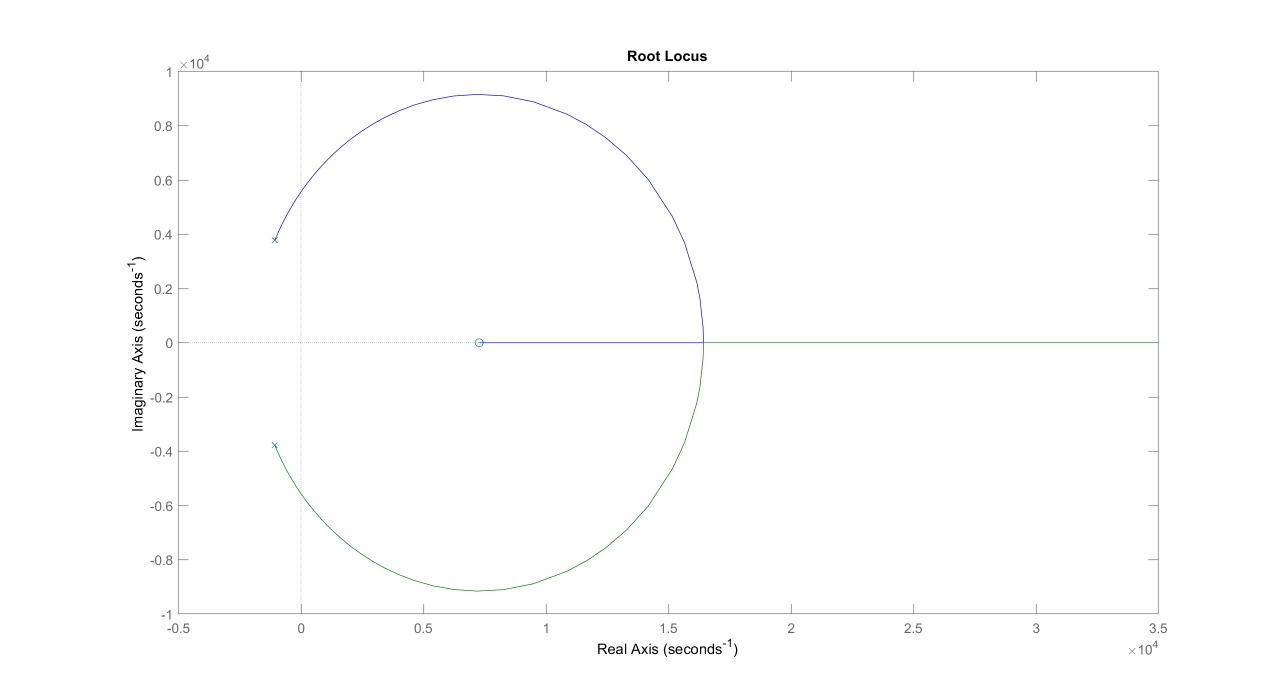
\includegraphics[scale=0.3]{Imagenes/Punto1/rootlocus_Convertidor.jpeg}
    \caption{ Mapa de raíces del convertidor Boost}
  \end{figure}


\subsubsection*{b) Valor real del Duty cycle}

El valor real de duty cycle obtenido de la simulaci\'on es $d_{real}=0.56$, mientras que el ideal es $d_{ideal}= \frac{V_o-V_1}{V_o}=0.6$.


El duty real no coincide con el ideal debido a que, cuando aumentamos la carga, aumenta el valor medio de la corriente en la inductancia, por lo que la ca\'ida de tensi\'on en el diodo es mayor. Del mismo modo, la ca\'ida de tensi\'on en la inductancia tambi\'en aumenta. Sumado a lo anterior, tenemos los efectos de la $ESR_L$. Todo esto contribuye a que la tensi\'on de salida $V_o$ se aleje del valor deseado y el duty te\'orico no sea el requerido en la pr\'actica.


\subsubsection*{c) Tiempos de establecimiento ante los cambios de carga }

Cuando ocurren cambios en la carga del circuito, la tensi\'on de salida de la fuente se ve afectada. Se midi\'o en LTspice el tiempo de establecimiento de la tensi\'on de salida al 5\% ante cambios de carga, para distintos valores de $R_6$. 

El tiempo que tarda en establecerse el circuito cuando la llave se abre (disminuci\'on de la carga) es mayor al tiempo que tarda en establecerse cuando la llave se cierra (aumento de la carga). A modo comparativo, solo se muestran acontinuaci\'on los gr\'aficos dichos tiempos cuando la llave se abre.  

\begin{figure}[H]
  \begin{subfigure}[b]{0.3\textwidth}
    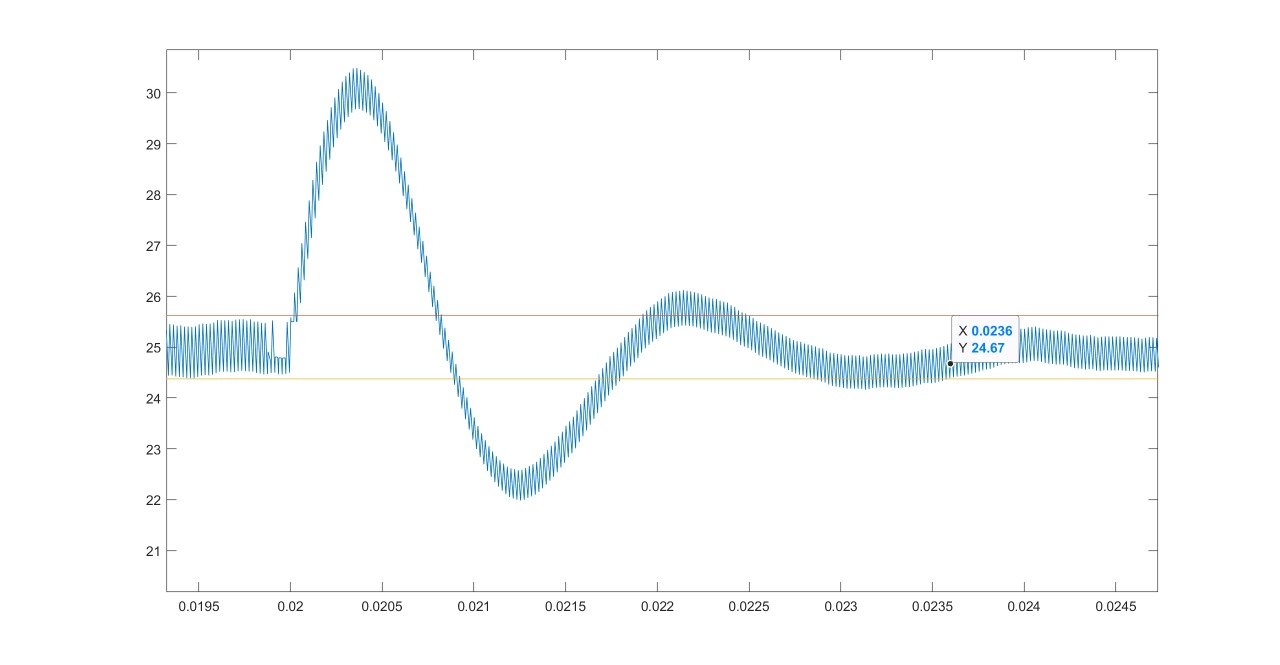
\includegraphics[width=\textwidth, height=\textwidth]{Imagenes/Punto1/Test_con_R6_1k.jpeg}
    \caption{ Con $R_6=1k\Omega$}
    \label{fig:f1}
  \end{subfigure}
  \hfill
  \begin{subfigure}[b]{0.3\textwidth}
    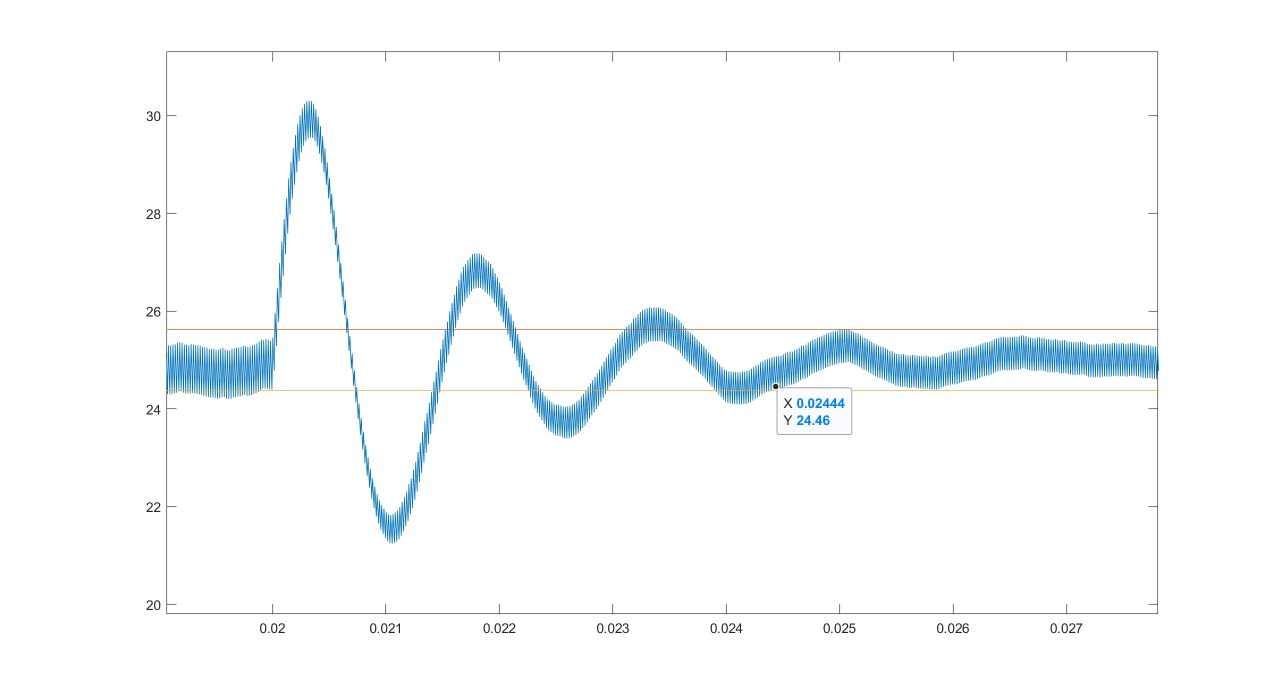
\includegraphics[width=\textwidth, height=\textwidth]{Imagenes/Punto1/Test_con_R6_10k.jpeg}
    \caption{ Con $R_6=10k\Omega$}
    \label{fig:f2}
  \end{subfigure}
  \hfill
  \begin{subfigure}[b]{0.3\textwidth}
    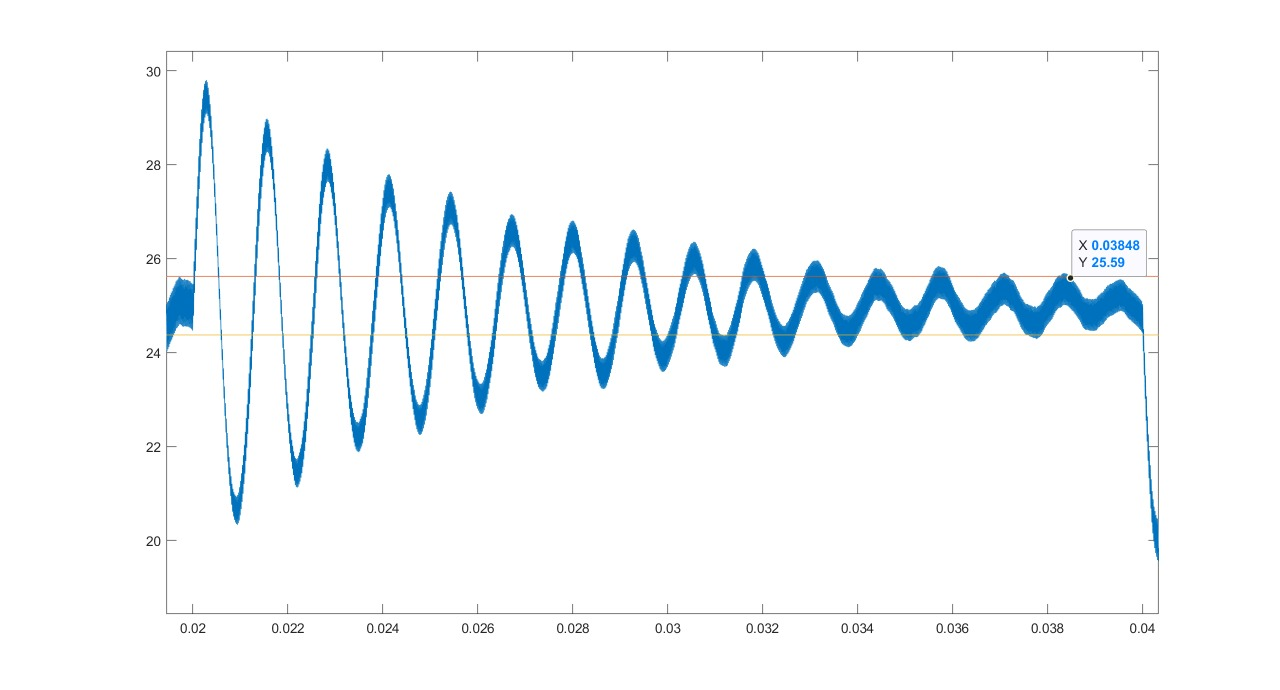
\includegraphics[width=\textwidth, height=\textwidth]{Imagenes/Punto1/Test_con_R6_22k.jpeg}
    \caption{ Con $R_6=22k\Omega$}
    \label{fig:f3}
  \end{subfigure}
  \caption{Tiempos de establecimiento ante los cambios de carga cuando la llave se abre}
  \label{osc}
\end{figure}

Los tiempos de establecimiento resultantes cuando la llave se abre son: 
\hspace{0.1cm}
\begin{equation}
t_e(R_6=1k\Omega)=3.6 mseg
\hspace{1cm}
t_e(R_6=10k\Omega)=4.44 mseg
\hspace{1cm}
t_e(R_6=22k\Omega)=18.48 mseg
\end{equation}

Para el caso de $R_6=10k\Omega$ tambi\'en se midi\'o el tiempo de establecimiento al 5\% cuando la llave se cierra resultando un 30\% menor a $t_e(R_6=10k\Omega)$. 

A partir de analizar la Figura \ref{osc}, notamos que medida que aumenta $R_6$, el tiempo de establecimiento es mayor. El sistema m\'as amortiguado resulta el de $R_6=1k\Omega$, luego le sigue $R=10k\Omega$ y, finalmente, el sistema de $R_6=22k\Omega$ con un movimiento ligeramente amortiguado. Los motivos por los cuales sucede esto ser\'an explicados acontinuaci\'on en el item d).

\subsubsection*{d) Diagramas de bode de la ganancia a lazo cerrado }

Una vez obtenida la ganancia a lazo cerrado del sistema en Matlab, procedemos a trazar el diagrama de bode y el diagrama de polos y ceros para los distintos valores de resistencia $R_6$, obteniendo los siguientes resultados:  
  
  \begin{equation}
  G_{\: lazo \:  cerrado}= \frac{\frac{ \widetilde{v_o}(s)}{\widetilde{d}(s)}}{1- \frac{ \widetilde{v_o}(s)}{\widetilde{d}(s)} \cdot \frac{\widetilde{v_c}(s)}{\widetilde{v_o}(s)} \cdot \frac{1}{9} }
  \end{equation}
  
\begin{figure}[H]
  \begin{subfigure}[b]{0.5\textwidth}
    \includegraphics[width=\textwidth, height=\textwidth]{Imagenes/Punto1/bode.png}
    \caption{ Diagrama de Bode de la ganancia a lazo cerrado}
    \label{fig:f12}
  \end{subfigure}
  \hfill
  \begin{subfigure}[b]{0.5\textwidth}
    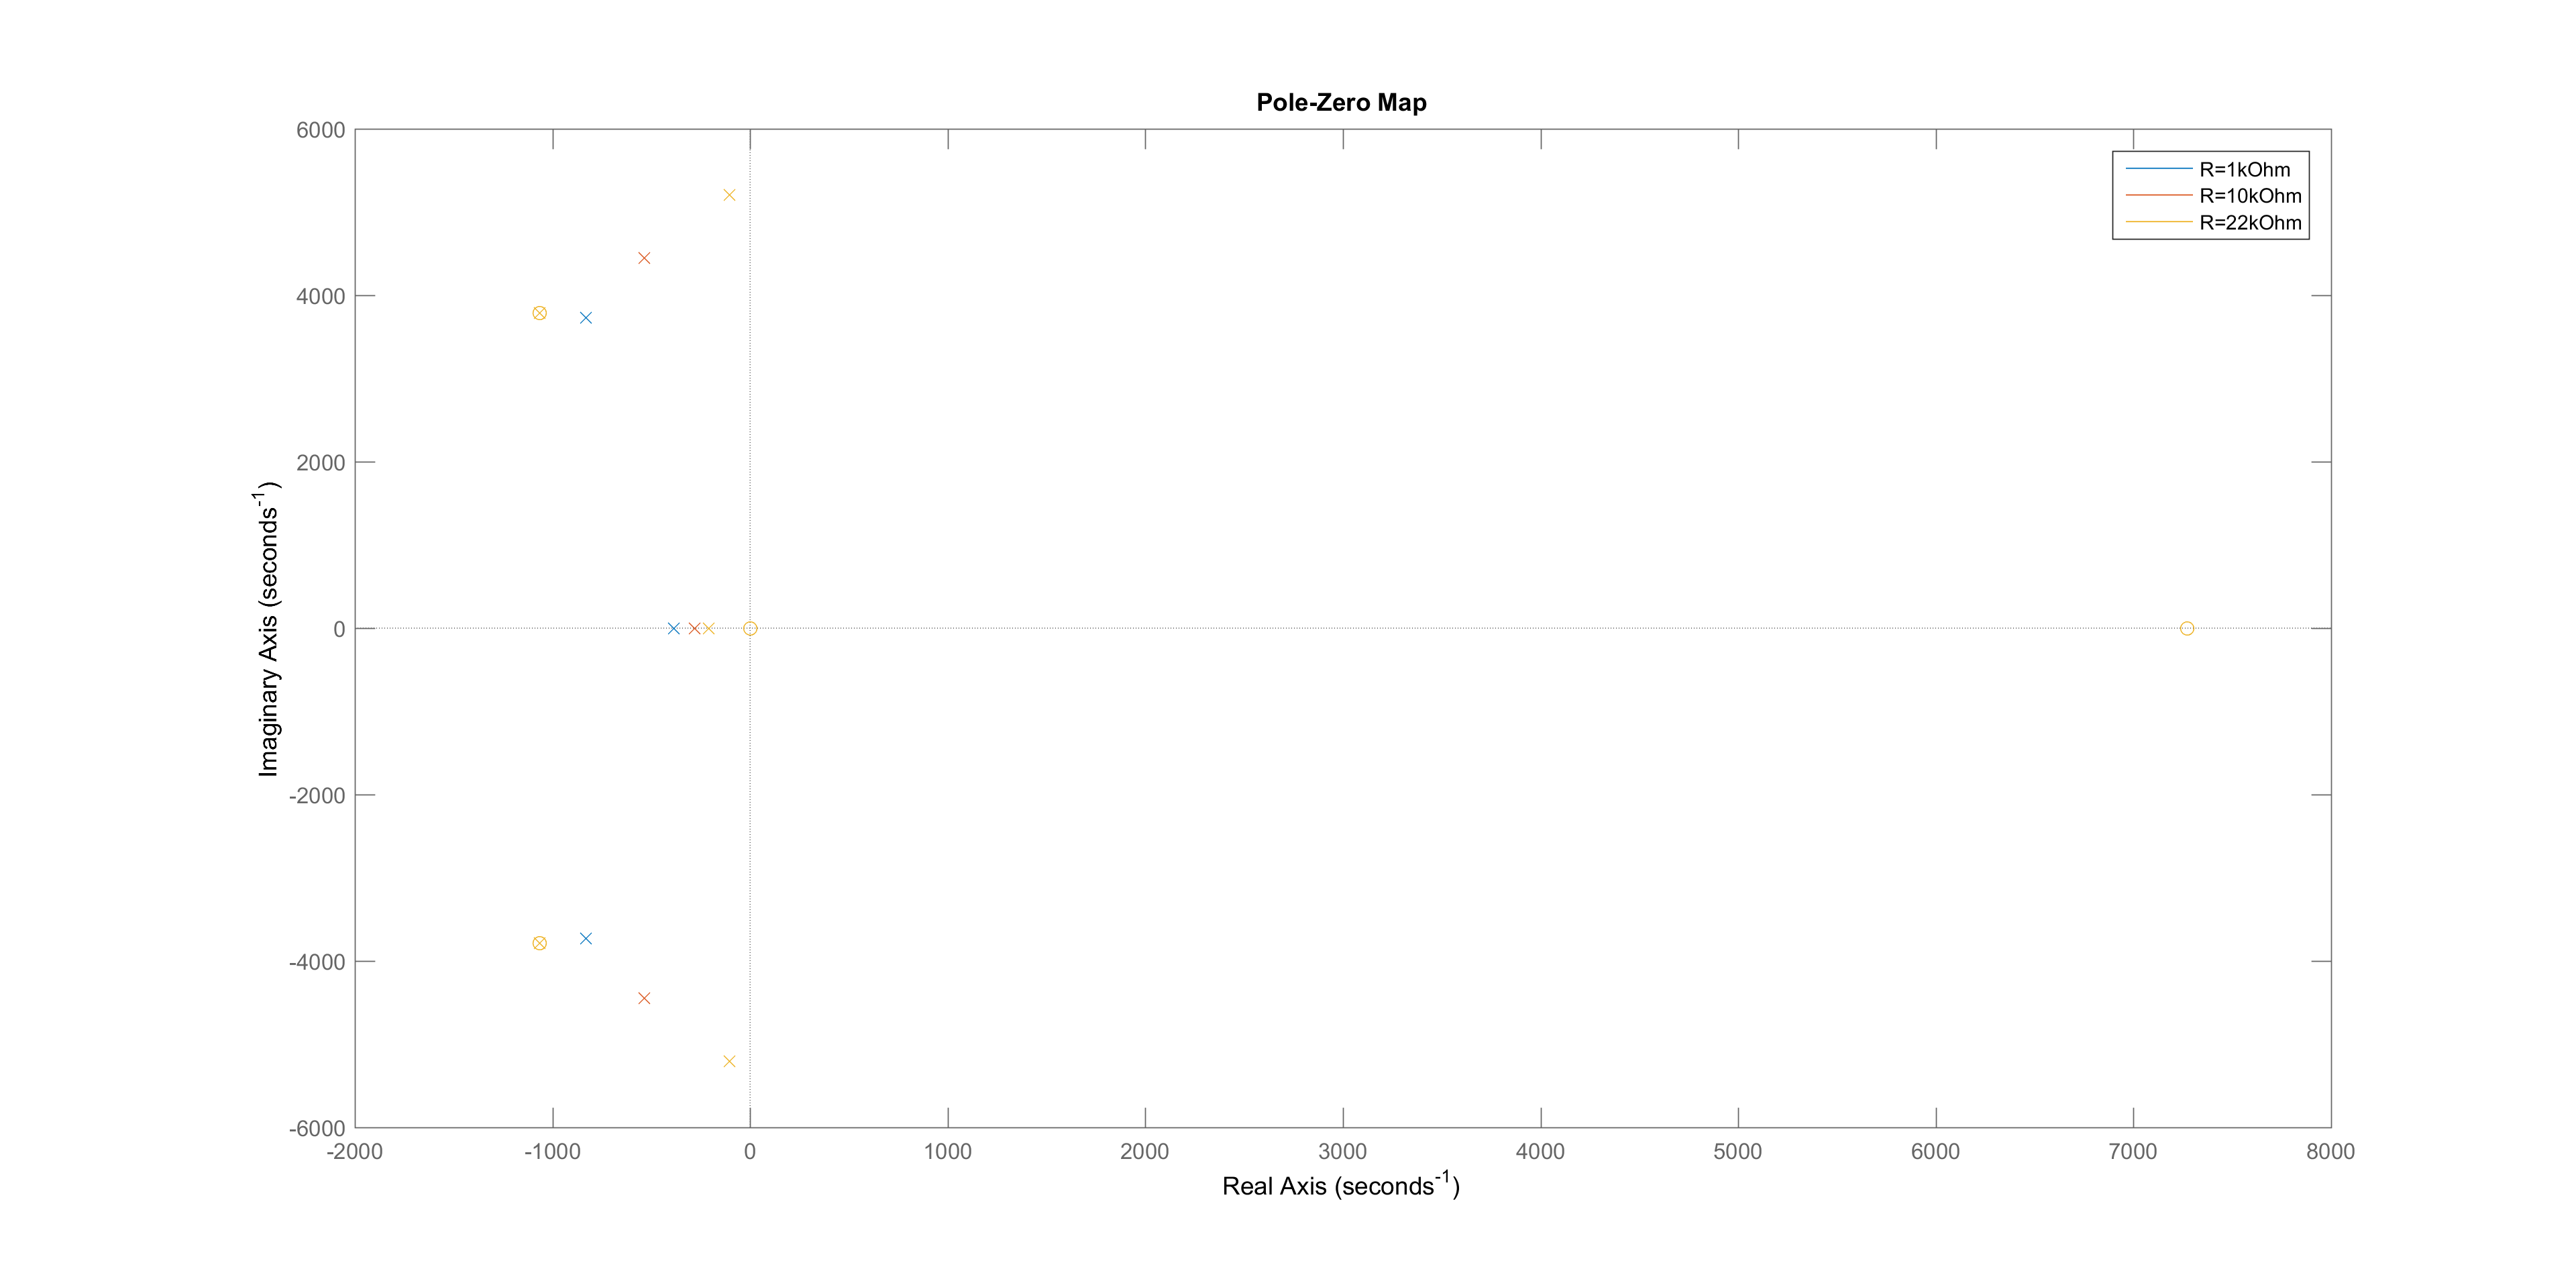
\includegraphics[width=\textwidth, height=\textwidth]{Imagenes/Punto1/polosyceros.png}
    \caption{ Diagrama de polos y ceros de la ganancia a lazo cerrado}
    \label{fig:f22}
  \end{subfigure}
\end{figure}  
  
  
A medida que aumentamos $R_6$, estamos aumentando la ganancia proporcional (Ver secci\'on 1.1.c) por lo que los polos del sistema se acercan cada vez m\'as al eje $jw$ haciendo tender el sistema a un sistema cada vez m\'as inestable. Este es el motivo por el cual los tiempos de establecimiento de la secci\'on anterior aumentaban a medida que $R_6$ se hacia m\'as grande. 

A partir del diagrama de bode, notamos que el factor de amortiguamiento aumenta a medida que disminuimos $R_6$, resultando en un sistema cada vez m\'as amortiguado.

Por último, vemos el análisis del margen de ganancia y del margen de fase para cada caso:
\begin{figure}[H]
  \begin{subfigure}[b]{0.5\textwidth}
    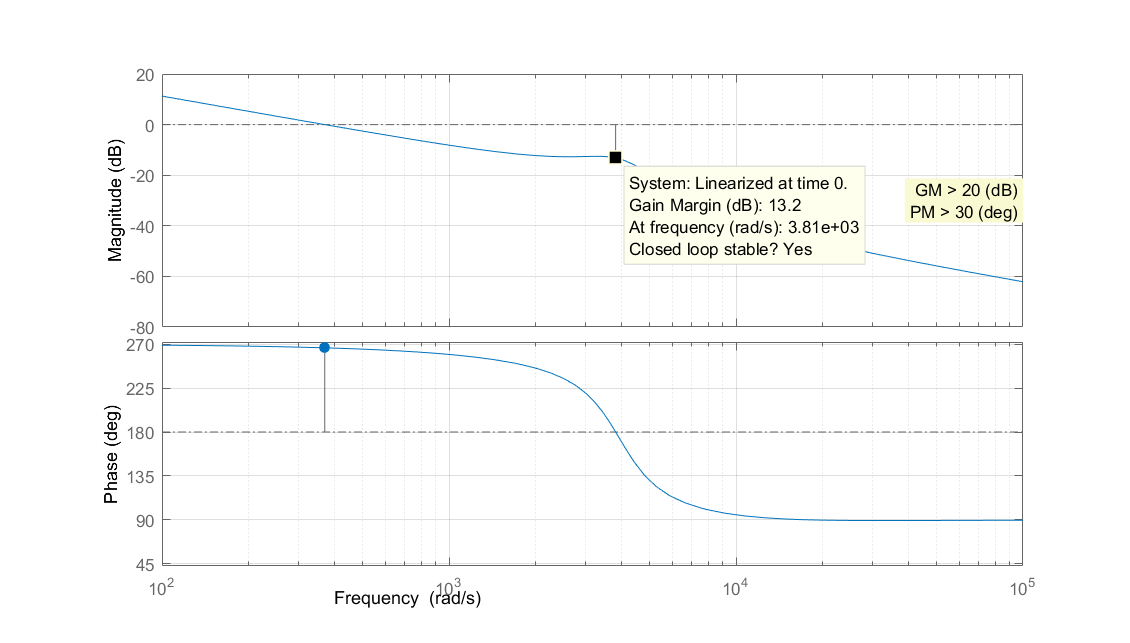
\includegraphics[width=\textwidth, height=\textwidth]{Imagenes/Punto1/fotosMarce/r1k.png}
    \caption{ Margen de ganancia y fase para $R=1 k\Omega $}
    \label{fig:f12}
  \end{subfigure}
  \hfill
  \begin{subfigure}[b]{0.5\textwidth}
    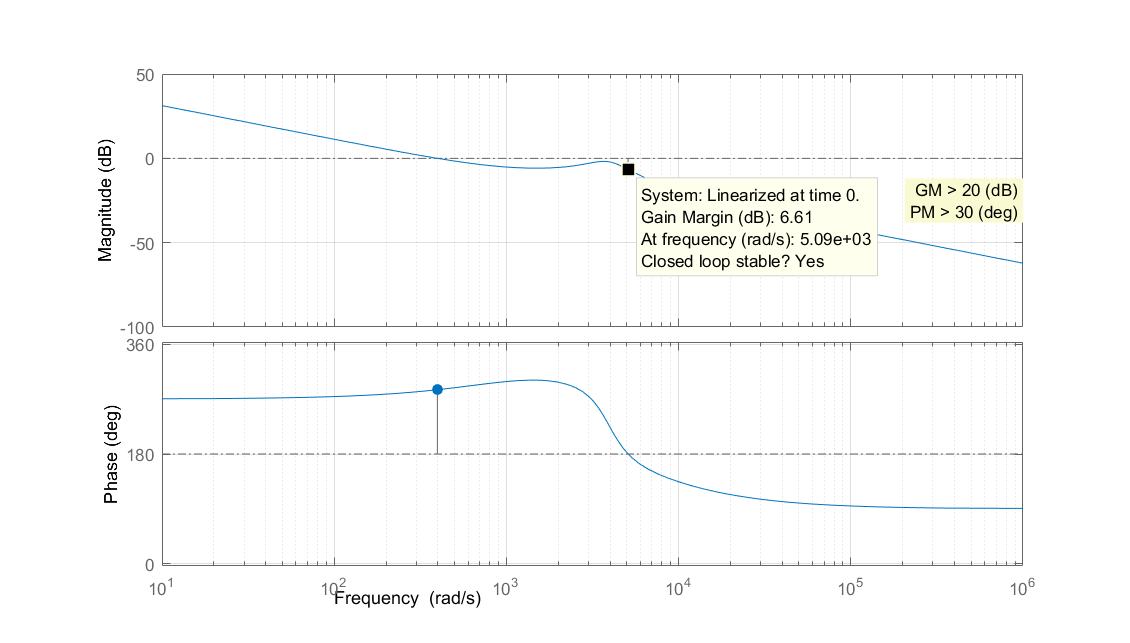
\includegraphics[width=\textwidth, height=\textwidth]{Imagenes/Punto1/fotosMarce/r10k.png}
    \caption{ Margen de ganancia y fase para $R=10 k\Omega $}
    \label{fig:f22}
  \end{subfigure}
	\hfill
  \begin{subfigure}[H] {0.5\textwidth}
  
    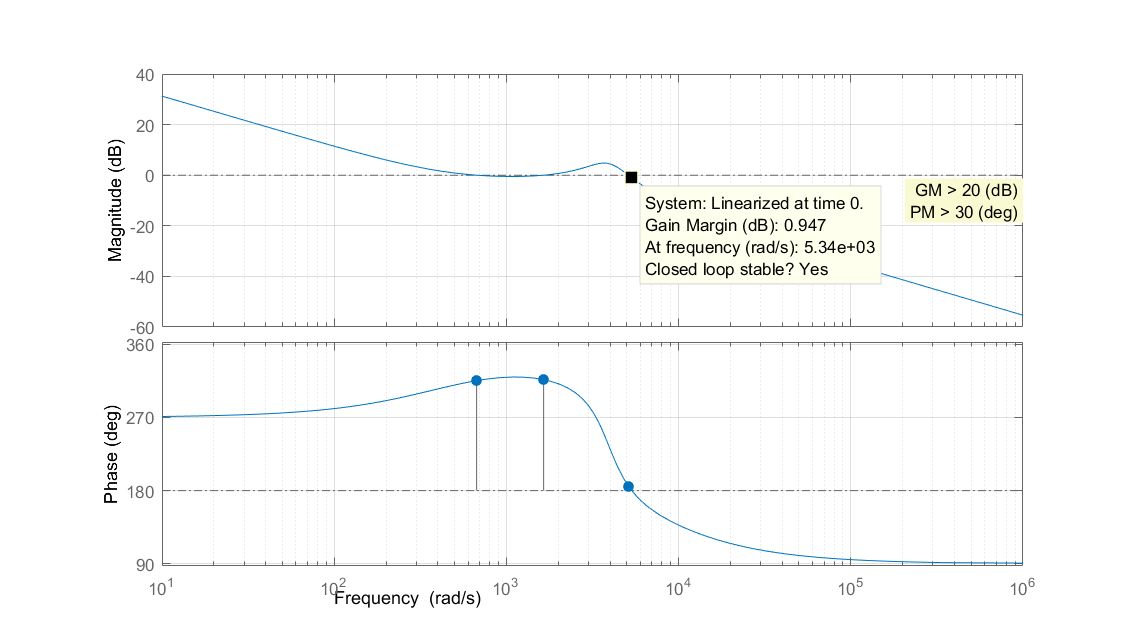
\includegraphics[width=\textwidth, height=\textwidth]{Imagenes/Punto1/fotosMarce/r22k.png}
    \caption{ Margen de ganancia y fase para $R=22 k\Omega$ }
      \label{fig:f13}
  \end{subfigure}

\end{figure}

Como podemos observar, a medida que R6 aumenta, el margen de ganancia va disminuyendo, por lo que el sistema tiende a ser inestable, como se observó en las respuestas temporales. Para los casos de $R_6$ simulados no se llega a dicha condición pero si bastante cerca.
\end{document}